\documentclass[class=report, crop=false, a4paper, 12pt]{standalone}

%Packages import
\usepackage{../pkgs}


\begin{document}
\newpage
% A face recognition system works in either or both of two modalities: face verification (or authentication) or face identification (or recognition). The difference between them lies in the final stage of the workflow, identification involves a one-to-one pairing, while identification is a one-to-many match.

\section{Face Recognition}
Face Recognition (FR) is a thoroughly debated and extensively researched task in the Computer Vision community for more than two decades \autocite{ranjanDeepLearningUnderstanding2018}, popularized in the early 1990s with the introduction of the Eigenfaces \autocite{turkEigenfacesRecognition1991} or Fisherfaces \autocite{p.n.belhumeurEigenfacesVsFisherfaces1997} approaches. These methods projected faces in a low-dimensional subspace assuming certain distributions, but lacked the ability to handle uncontrolled facial changes that broke said assumptions, henceforth, bringing about face recognition approaches through local-features \autocite{chengjunliuGaborFeatureBased2002, ahonenFaceDescriptionLocal2006} that, even though, presented considerable results, weren't distinctive or compact. Beginning in 2010, methods based on learnable filters arose \autocite{z.caoFaceRecognitionLearningbased2010,leiLearningDiscriminantFace2014}, but unfortunately revealed limitations when nonlinear variations were at stake.

\par Earlier methods for FR worked appropriately when the data was handpicked or generated on a constrained environment, however, they didn't scale adequately in the real world were there are large fluctuations in, particularly, pose, age, illumination, background scenario, the presence of facial occlusion \autocite{ranjanDeepLearningUnderstanding2018} and many unimaginable more. These shortcomings can be dealt with by using Deep Learning, a framework of techniques that solves the nonlinear inseparable classes problem \red{ref.}, more specifically a structure called Convolutional Neural Network (CNN) \autocite{wangDeepFaceRecognition2021}. 

\par CNNs are an Artificial Neural Network (ANN) that exhibit a better performance on image or video-based tasks compared to other methods \autocite{lecunGradientBasedLearningApplied1998}. They were greatly hailed in 2012, after the AlexNet \autocite{krizhevskyImageNetClassificationDeep2012} victory, by a great margin, in the ImageNet Large Scale Visual Recognition Challenge (ILSVRC). Just two years later, DeepFace \autocite{taigmanDeepFaceClosingGap2014} revolutionized the benchmarks scores by achieving state-of-the-art results that approached human performance, reinforcing even further the importance of Deep Learning and shifting the research path to be taken \autocite{wangDeepFaceRecognition2021}.

\par Given what has been stated so far and the proven robustness, performance, and overall results in computer vision \red{ref. won competitions}, the methods discussed in this dissertation will therefore deal exclusively with Deep Learning approaches. For more information on other methods, please refer to \autocite{learned-millerLabeledFacesWild2016}.
% The exponential growth in the Artificial Intelligence domain, its corresponding subfields and technologies involved, spanned a plethora of terms that can be easily confused, mistook or mixed. For a better understanding of this dissertation, before discussing methods and implementations, it's important to analyze the fundamentals.


% \vspace{\baselineskip}
% \noindent\textbf{Computer Vision} is the science of trying to mimic with a computer what the humans do when looking at a scene, that is, extracting information from images through a series of computational techniques. \autocite{szeliskiComputerVisionAlgorithms2022}

% \vspace{\baselineskip}
% \noindent\textbf{Image querying}, is the process of finding information in a database of images that corresponds to the user query\footnote{Query, in computer science, is the request for information in a database.}, in this case, an image query\autocite{bartoliniImageQuerying2009}.  

% \vspace{\baselineskip}
% \noindent\textbf{Face verification}, also referred to as \textbf{face authentication}, is a one-to-one match, and it's the action of verifying if the query face matches the identity that's being claimed. These principles are used in biometric systems such as self-service immigration clearance using E-passport. \autocite{liHandbookFaceRecognition2011}

% \vspace{\baselineskip}
% \noindent\textbf{Face identification}, also called \textbf{face recognition}, is a one-to-many correlation process that compares a query face to a database of faces and associates it to the corresponding match (or matches). A typical use case is to identify someone in a watchlist or surveillance videos. \autocite{liHandbookFaceRecognition2011} 

\section{A Face Recognition System}
\par According to Ranjan \textit{et al.} \autocite{ranjanDeepLearningUnderstanding2018}, the goal of a FR system is to find, process and learn from a face, gathering as much information as possible, and as a result, it is one of the most widely implemented biometric system solutions, in light of its versatility when facing real world application \autocite{duElementsEndtoendDeep2022}, such as \red{military, public security and daily life}.

\par By and large, all end-to-end automatic face recognition systems follow a sequential and modular\footnote{Sequential because each stage relies on the output from the previous ones, and modular in the sense that each stage employs its own method and it can be modified to better adapt to specific tasks.} pipeline \reffig{fig:fr pipeline} composed of three pillar stages \autocite{wangDeepFaceRecognition2021}: face detection, face alignment and face representation. First an image or video feed is used as an input then, as the name suggests, the \textbf{face detection} module is responsible for finding a face. Next, the \textbf{face alignment} phase applies spatial transformations to the data in order to normalize the faces' pictures (or frames, in the case where a video is used) to a standardized view. Finally, the \textbf{face representation} stage, makes use of deep learning techniques to learn discriminative features that will allow the recognition.

\par All three stages have their individual importance and methods of implementation\footnote{For a deeper and extensive study, please refer to: \autocite{zafeiriouSurveyFaceDetection2015} in the case of classic face detection approaches and \autocite{minaeeGoingDeeperFace2021} for deep learning based methods; \autocite{wangFacialFeaturePoint2018} addresses traditional face alignment methods and is complemented with \autocite{duElementsEndtoendDeep2022} for more up-to-date techniques; and \autocite{learned-millerLabeledFacesWild2016} tackles classic face representation \red{(add the following if needed) while X supplements the deep learning ones.}}. Face detection is achievable through classical approaches \autocite{violaRapidObjectDetection2001, brubakerDesignCascadesBoosted2008} or deep methods, among them is \autocite{dengRetinaFaceSinglestageDense2019} and the widely applied \autocite{zhangJointFaceDetection2016a}. Face alignment, once again, can be accomplished through traditional measures \autocite{cootesViewbasedActiveAppearance2002, martinezLocalEvidenceAggregation2013} or more modern ones, namely \autocite{huangPropagationNetPropagatePoints2020} or the aforementioned \autocite{zhangJointFaceDetection2016a} which concurrently performs detection and alignment. To conclude, the face representation module is no exception, and can also be divided in two groups, regarding the methodology used. Some conventional systems were already mentioned, such as \autocite{p.n.belhumeurEigenfacesVsFisherfaces1997,turkEigenfacesRecognition1991}, and the deep learning ones are the object of discussion of this dissertation and will be reviewed along the following sections, therefore, the focus will be on describing, with particular interest, the face representation stage.

\begin{figure}[!t]
    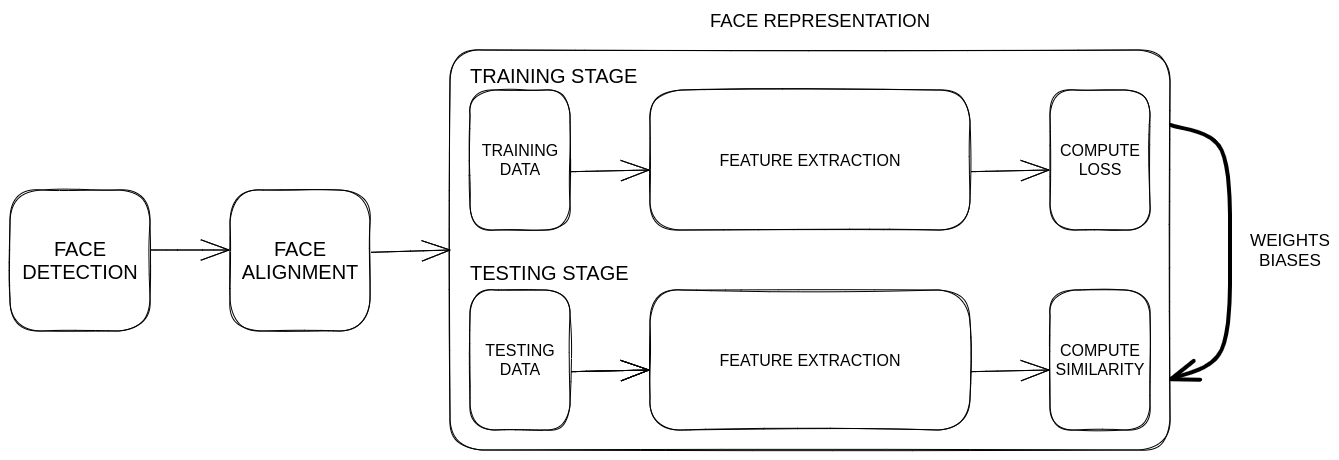
\includegraphics[scale=0.30]{fr_pipeline.png}
    \caption[Pipeline]{A typical face recognition pipeline, guided by the approach in \autocite{wangDeepFaceRecognition2021}.}
    \label{fig:fr pipeline}
\end{figure}

\subsection{Face Detection}
\par Face detection is the first step in any automatic facial recognition system. Given an input image to a face detector module, it is in charge of detecting every face in the picture and returning bounding-boxes coordinates, for each one, with a certain confidence score \autocite{duElementsEndtoendDeep2022,ranjanDeepLearningUnderstanding2018}.

\par Previously employed traditional face detectors \red{cite here} are incapable of detecting facial information when faced with challenges such as variants in image resolution, age, pose, illumination, race, occlusions or accessories (masks, glasses, makeup) \autocite{duElementsEndtoendDeep2022,ranjanDeepLearningUnderstanding2018}. The progress in deep learning and increasing GPU power led DCNNs to become a viable and reliable option that solves said problems in face detection. 

\par These techniques can be included in different categories. A more analytical perspective \autocite{duElementsEndtoendDeep2022} distributes the methods, depending upon their architecture or purpose of application, over seven categories: multi-stage, single-stage, anchor-based, anchor-free, multi-task learning, CPU real-time and, finally, problem-oriented. Additionally, being as the face detection problem can be seen as a specific task in a general object detection situation, it is no surprise that several works inherit from them and, therefore, some bases are referenced throughout the next list.

\vspace{0.5\baselineskip}
\begin{figure}[h!]
    \centering
    \begin{minipage}[c]{0.38\textwidth}
      \centering
      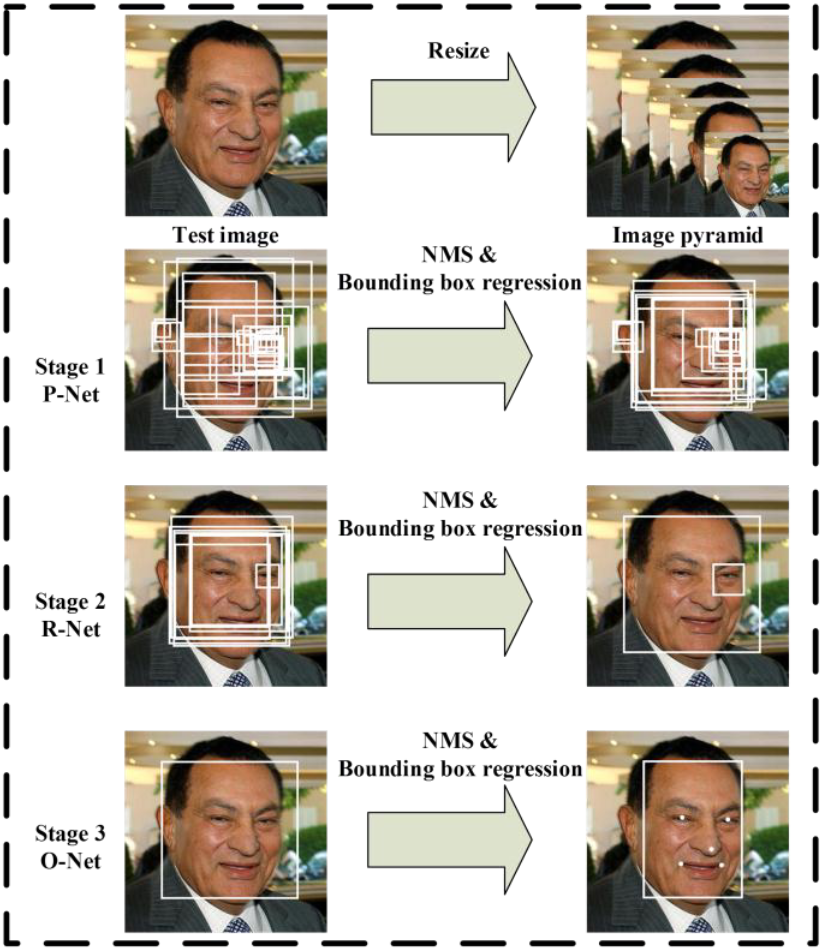
\includegraphics[width=\textwidth]{mtcnn.png}
      \label{fig:mtcnn}
    \end{minipage}
    \hspace{0.5cm}
    \begin{minipage}[c]{0.52\textwidth}
      \centering
      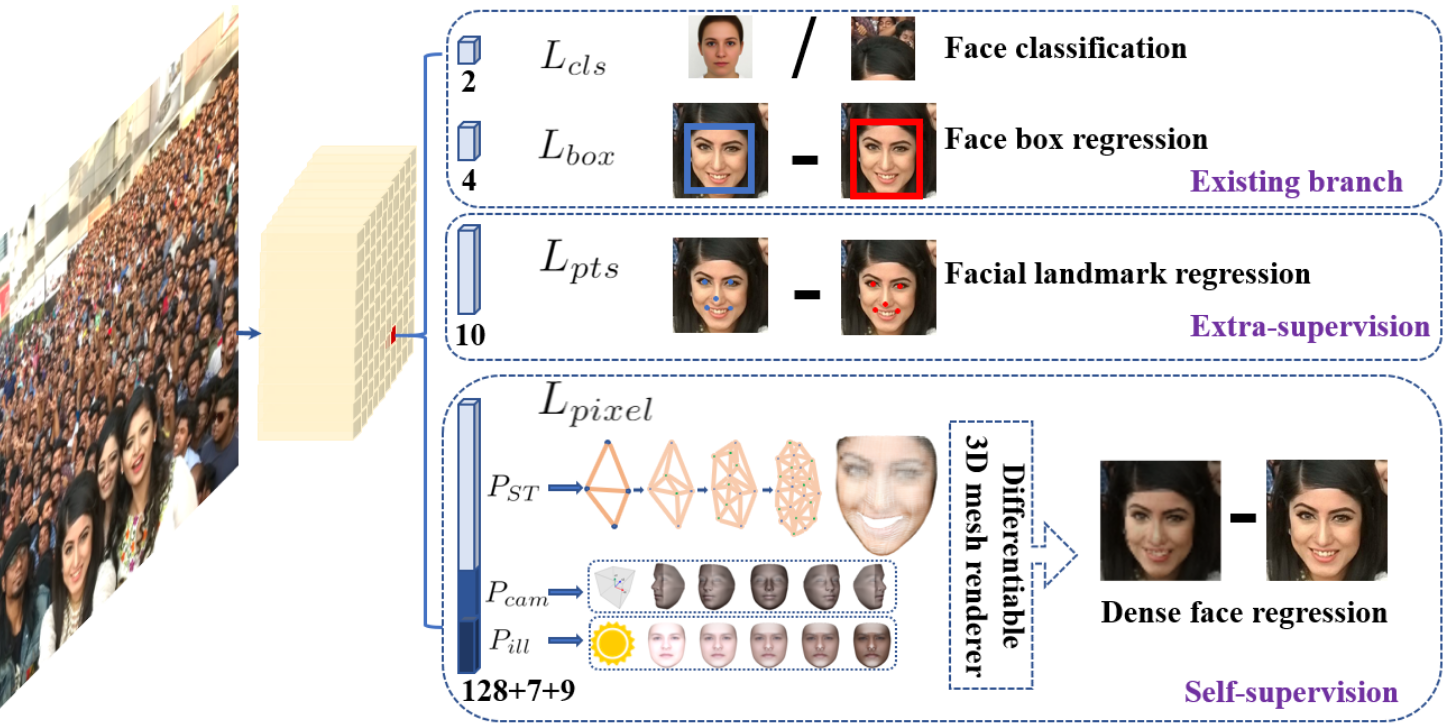
\includegraphics[width=\textwidth]{retinaface.png}
      \label{fig:retinaface}
    \end{minipage} 
    \begin{minipage}{0.4\textwidth}
        \vspace{-0.5cm}
        \centering
        \footnotesize a)
    \end{minipage}
    \hfill
    \begin{minipage}{0.4\textwidth}
        \vspace{-0.5cm}
        \centering
        \footnotesize b)
    \end{minipage}
    \vspace{-0.4cm}
    \caption{Comparison between \textbf{a)} MTCNN: multi-stage, CPU real-time and multi-task learning, and \textbf{b)} RetinaFace: single-stage, anchor-based, CPU real-time and multi-task learning. MTCNN \autocite{zhangJointFaceDetection2016a} proposes a series of bounding boxes then, through a series of refinement stages, the best solution and landmarks are found. RetinaFace \autocite{dengRetinaFaceSinglestageDense2019} accomplishes, in a single-stage, face classification and bounding box regression by evaluating anchors, landmark localization and dense 3D projection for facial correspondence.}
    \label{fig:mtcnn vs retinaface}
\end{figure}
  

\par \noindent \textbf{Multi-stage} methods \autocite{dengRetinaFaceSinglestageDense2019} include all the coarse-to-fine facial detectors that work in similar manner to the following two phases. First, bounding box proposals are generated by sliding a window through the input. Then, over one or several subsequent stages, false positives are rejected and the approved bounding boxes are refined. To complement, one widely applied object detection protocol that inspired face detection methods and perfectly describes the steps mentioned above is Faster R-CNN \autocite{renFasterRCNNRealTime2016}. However, these methods can be slower and have a more complex way of training \autocite{xuCenterFaceJointFace2019}.

\vspace{\baselineskip}
\par \noindent \textbf{Single-stage} approaches \autocite{dengRetinaFaceSinglestageDense2019} are the ones that perform classification and bounding box regression without the necessity of a proposal stage, producing highly dense face locations and scales. This structure takes inspiration, once again, from general object detectors, for example, the Single Shot MultiBox detector, commonly referred to as SSD \autocite{liuSSDSingleShot2016}. Finally, the methods included in this class are more efficient, but can incur in compromised accuracy, when compared to multi-stage.

\vspace{\baselineskip}
\par \noindent \textbf{Anchor-based} techniques \autocite{liuHAMBoxDelvingOnline2019, dengRetinaFaceSinglestageDense2019, zhangFaceDetectionUsing2018} detect faces by predefining anchors with different settings (scales, strides, number, etc.) on the feature maps, then performing classification and bounding box regression on them until an acceptable output is found. As proven by Liu and Tang \textit{et al.} \autocite{liuHAMBoxDelvingOnline2019}, the choice of anchors highly influences the results of prediction. Hence, it is necessary to fine-tune them on a situation-by-situation basis, otherwise, there is a limitation in generalization. Furthermore, higher densities of anchors directly generate an increase in computational overhead.

\vspace{\baselineskip}
\par \noindent \textbf{Anchor-free} procedures, obviously, do not need predefined anchors in order to find faces. Alternatively, these methods address the face detection by using different techniques. For example, DenseBox \autocite{huangDenseBoxUnifyingLandmark2015} which attempts to predict faces by processing each pixel as a bounding box, or CenterFace \autocite{xuCenterFaceJointFace2019} that treats face detection as a key-point estimation problem by predicting the center of the face and bounding boxes. Even so, relating to the accuracy of anchor-free approaches, there's still room for improvement for false positives and stability in the training stage \autocite{duElementsEndtoendDeep2022}.

\vspace{\baselineskip}
\phantomsection\label{mt learning}
\par \noindent \textbf{Multi-task learning} are all the methodologies that conjointly performs other tasks, namely facial landmark\footnote{A facial landmark is a key-point in a face that contributes with important geometric information, namely the eyes, nose, mouth, etc. \autocite{fengWingLossRobust2018}} localization, during face classification and bounding box regression \autocite{duElementsEndtoendDeep2022}. CenterFace \autocite{xuCenterFaceJointFace2019} is one example, and so it is the widely implemented MTCNN \autocite{zhangJointFaceDetection2016a}, which correlated bounding boxes and face landmarks. RetinaFace \autocite{dengRetinaFaceSinglestageDense2019} is another state-of-the-art approach, it mutually detects faces, respective landmarks and performs dense 3D face regression.

\vspace{\baselineskip}
\par \noindent \textbf{CPU real-time} methods, as the name suggests, include the detectors that can run on a single CPU core, in real-time, for VGA-resolution input images. A face detector can achieve great results in terms of accuracy, but for real world applications, its use can be too computational heavy, therefore, can't be deployed in real time (specially in devices that do not have a GPU) \autocite{duElementsEndtoendDeep2022}. MTCNN \autocite{zhangJointFaceDetection2016a}, Faceboxes \autocite{zhangFaceBoxesCPURealtime2018}, CenterFace \autocite{xuCenterFaceJointFace2019} or RetinaFace \autocite{dengRetinaFaceSinglestageDense2019} are examples of this category.

\vspace{\baselineskip}
\par \noindent \textbf{Problem-oriented} is a category that includes the detectors that are projected to resolve a wide range of specific problems, for example, faces that are tiny, partially occluded, blurred or scale-invariant face detection \autocite{duElementsEndtoendDeep2022}. PyramidBox \autocite{tangPyramidBoxContextassistedSingle2018} is an example that solves the partial occluded and blurry faces, and HR \autocite{huFindingTinyFaces2017} tackles the tiny faces challenge.

\vspace{\baselineskip}
Although this distribution can create some overlap among the categories, it is superior due to the simplicity of inferring what defines each category and being a more fine-grained way of classifying techniques when compared to others, namely the dual categorical division by \autocite{ranjanDeepLearningUnderstanding2018} that groups the methods in region\footnote{Region-based approaches creates thousands of generic object-proposals for every image, and subsequently, a DCNN classifies if a face is present in any of them.} or sliding-window\footnote{Sliding-window approaches centers on using a DCNN to compute a face detection score and bounding box at every location in a feature map.} based. 

\subsection{Face Alignment}
\par Face Alignment, or facial landmark detection \autocite{changFacePoseNetMakingCase2017}, is the second stage of the face recognition pipeline, and has the objective of calibrating the detected face to a canonical layout, through landmark-based or landmark-free approaches, in order to leverage the core final stage of face representation \autocite{duElementsEndtoendDeep2022}. 
\par Despite the fact that traditional face alignment methods are very accurate, that only occurs in constrained circumstances. Therefore, once again, to address that issue, deep learning-based methods are the solution to perform an accurate facial landmark localization that realistically scales to real world scenarios \autocite{fengWingLossRobust2018}. 
\par Furthermore, face alignment, can be accomplished through two categories of methods: landmark-based and landmark-free.

\vspace{\baselineskip}
\par \noindent \textbf{Landmark-based alignment} is a category of methods that exploits the facial landmarks with the aim of, through spatial transformations, calibrating the face to an established layout \autocite{duElementsEndtoendDeep2022}. This can be accomplished through: coordinate regression, heatmap regression or 3D Model Fitting. \textbf{Coordinate regression-based} methodologies \autocite{fengWingLossRobust2018,liuTwoStreamTransformerNetworks2018,zhangJointFaceDetection2016a} consider the landmark localization as a numerical objective, i.e. a regression, thus an image is fed to a DCNN and it will output a vector of landmark coordinates. \textbf{Heatmap Regression} \autocite{dengJointMultiviewFace2017,wuLookBoundaryBoundaryAware2018,chenFaceAlignmentKernel2019} is different from coordinate regression because, although it is a numerical objective task, the output is not a coordinate vector, but a map of likelihood of landmarks' locations. Finally, \textbf{3D Model Fitting} \autocite{bhagavatulaFasterRealtimeFacial2017,changFacePoseNetMakingCase2017,xiaoRecurrent3D2DDual2017}is the category that integrates methods that consider the relation between 2D facial landmarks and the 3D shape of a generic face. The particularity of them is the reconstruction of the 3D face from a 2D face image that is then projected over a plane in order to obtain the landmarks. 

\vspace{\baselineskip}
\par \noindent \textbf{Landmark-free alignment}, on the other hand, integrates the approaches that do not rely on landmarks as a reference to align the face, in contrast, these type of methods incorporate the alignment into a DCNN that gives, as a result, an aligned face \autocite{duElementsEndtoendDeep2022}. An example of an end-to-end method that does not depend on facial landmarks is RDCFace \autocite{zhaoRDCFaceRadialDistortion2020}, and it rectifies distortions, applies alignment transformations and executes face representation. Hayat et al. \autocite{hayatJointRegistrationRepresentation2017} proposes a method that deals with extreme head poses. The process to register faces in an image with high pose variance can be quite challenging and often demands complex pre-processing, namely landmark localization, therefore, to address that, a DCNN is employed that does not rely on landmark localization and concomitantly register and represent faces.

%A facial landmark is nothing more than an important geometric point of reference that facilitates the alignment by acting as a reference

\vspace{\baselineskip}
\par As can be seen from the previous section, this step in the face recognition process can be accomplished, very sporadically, through standalone methods that process the detected face from the previous stage, but generally joint detection and alignment methods (and sometimes even face representation), previously referenced in the \hyperref[mt learning]{multi-task learning} definition, are the optimal choice \autocite{changFacePoseNetMakingCase2017}.

\subsection{Face Representation}

\newpage
\section{Face Representation Pipeline}


\subsection{Convolutional Neural Networks} %Review this article \autocite{kangDeepSimilarityMetric2019}
There are several types of Neural Networks architectures, but Convolutional Neural Networks (CNNs or Convnets) are probably the most widely implemented model overall \autocite{yamashitaConvolutionalNeuralNetworks2018, liSurveyConvolutionalNeural2022} with successful applications in the domains of Computer Vision \autocite{krizhevskyImageNetClassificationDeep2012,taigmanDeepFaceClosingGap2014,tompsonEfficientObjectLocalization2015, zhangImprovedBreastCancer2021} or Natural Language Processing\autocite{abdel-hamidConvolutionalNeuralNetworks2014, wangGenCNNConvolutionalArchitecture2015, xiangConvolutionalNeuralNetworkbased2020}. In the CNN category itself there are different variants, but they all abide the fundamental structure of a feedforward hierarchical multi-layer network \reffig{fig:cnn}. Feedforward because the information only flows in a singular direction without cycling \autocite{zellSimulationNeuronalerNetze1994}, hierarchical because the higher complexity internal representations are learned from lower ones \autocite{lecunDeepLearning2015, zhuBCNNBranchConvolutional2017} and multi-layer because it is composed of a series of stages, blocks or layers: the raw data is fed to an input layer, forwarded to a sequence of intercalating convolutional and pooling layers, transmitted to a stage of one or more fully-connected layers \autocite{lecunDeepLearning2015, yamashitaConvolutionalNeuralNetworks2018, guRecentAdvancesConvolutional2018, alzubaidiReviewDeepLearning2021}. The convolutional layer is designed to extract feature representations by being composed of kernels (or filter banks \autocite{lecunDeepLearning2015}) that compute feature maps through element-wise product, to which is applied a nonlinear activation function \autocite{guRecentAdvancesConvolutional2018,yamashitaConvolutionalNeuralNetworks2018}. Next is the pooling layer, that's responsible for reducing the spatial size of the input data \autocite{guRecentAdvancesConvolutional2018} and joining identical features \autocite{lecunDeepLearning2015}. Finally, the fully connected layers, and their core function is to perform high logic and generate semantic information \autocite{guRecentAdvancesConvolutional2018}.

\begin{figure}[t!]
    \centering
    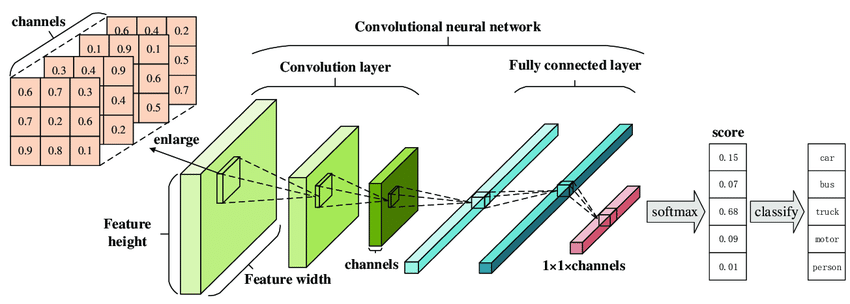
\includegraphics[width=0.85\textwidth]{Architecture-of-a-Convolutional-Neural-Network-CNN-The-traditional-CNN-structure-is.png}
    \caption{Architecture of a Convolutional Neural Network \autocite{kangDeepSimilarityMetric2019}.}
    \label{fig:cnn}
\end{figure}

\par Using CNNs for Computer Vision tasks is not an arbitrary choice, but due to the fact that the network design can benefit from the intrinsic characteristics of the input data, consequently performing really well in image related applications \autocite{lecunDeepLearning2015,caoReviewNeuralNetworks2018}. In the first place, images have an array-like structure with numerous elements, namely, each pixel has an assigned value organized in a grid-like manner \autocite{yamashitaConvolutionalNeuralNetworks2018}. In the second place, there's an inherent correlation between local groups of values, which creates distinguishable motifs \autocite{lecunDeepLearning2015}. Finally, the local values of images are invariant to location, that is, a certain composition should have the same value independently of the spatial location in the picture \autocite{lecunDeepLearning2015}. Therefore, the following key, unique features potentiate the previously stated efficient performance \autocite{caoReviewNeuralNetworks2018}:
\begin{enumerate}
    \item Designed to process multidimensional arrays \autocite{lecunDeepLearning2015};
    \item Shared weights between the same features in different locations; %Invariance to shift, distortions and rotations
    \item Automatically identifies the relevant features without any human supervision, hence, small amounts of preprocessing \autocite{alzubaidiReviewDeepLearning2021,liSurveyConvolutionalNeural2022}; %Easier to train
    \item Local connections (or receptive fields/sparse connectivity) \autocite{alzubaidiReviewDeepLearning2021}; %Less complexity, easier to train; %Invariance to shift, distortions and rotations and less network complexity (easier to train)
    \item Pooling layers that reduces the spatial size of the input data. %Invariance to shift, distortions and rotations
\end{enumerate}
% Check this article for better description of key features \autocite{liSurveyConvolutionalNeural2022}

The ensemble of features 2, 4 and 5 enable an invariance of the network to small shifts, distortions and rotations \autocite{guRecentAdvancesConvolutional2018,lecunDeepLearning2015}, while 2, 3, 4 and 5 helps to reduce the complexity of the model, and as a result training it is easier\autocite{guRecentAdvancesConvolutional2018,liSurveyConvolutionalNeural2022}.
\end{document}